\chapter{有资源预算的智能体任务调度}
\label{chap:scheduler}

\section{把计算组织成有向无环图}
一次结构解析通常包含多个候选：不同相位初值、空间群、晶畴模型或原子指派。它们能够共享输入，但不一定相互依赖。用有向无环图 $G=(V,E)$ 表示计算，节点 $v$ 是一次有明确输入和输出的动作，边 $u\to v$ 表示 $v$ 必须读取 $u$ 的结果。普通节点的就绪条件是
\begin{equation}
v\in\mathcal R\quad\Longleftrightarrow\quad
v\text{ 尚未执行，且 }\operatorname{pred}(v)\text{ 全部成功完成}.
\end{equation}
任务图因此同时说明了\textbf{哪些计算可以并行}和\textbf{结果从哪里来}。模型建议执行一个动作，调度器仍会检查它是否就绪、引用是否属于声明的依赖、输入文件是否与保存的哈希一致。

\begin{figure}[!htbp]
\centering
\begin{tikzpicture}[node distance=9mm and 13mm,>=Latex,
 box/.style={draw=ink!50,fill=pale,rounded corners=2pt,text width=39mm,minimum height=10mm,align=center,font=\small}]
\node[box] (inputs) {冻结的输入快照};
\node[box,below left=of inputs] (a) {候选 A 的原生精修};
\node[box,below right=of inputs] (b) {候选 B 的原生精修};
\node[box,below=27mm of inputs] (review) {汇集结果及失败证据};
\node[box,below=of review] (package) {校验并打包产物};
\draw[->] (inputs)--(a);\draw[->] (inputs)--(b);
\draw[->] (a)--(review);\draw[->] (b)--(review);
\draw[->] (review)--(package);
\end{tikzpicture}
\caption{双起点精修的依赖关系。输入在会话初始化时保存；两个精修动作独立执行，汇总节点等待二者结束。汇总成功表示证据已汇集，并不自动宣布某个结构成立。}
\end{figure}

\section{资源约束是明确的加法}
令正在执行的节点集合为 $\mathcal A$，节点申请的线程数和内存额度分别为 $c_v,m_v$。调度器只在以下条件同时成立时接纳一个新任务：
\begin{equation}
|\mathcal A|\le W,\qquad
\sum_{v\in\mathcal A}c_v\le C,\qquad
\sum_{v\in\mathcal A}m_v\le M.
\label{eq:resource-admission}
\end{equation}
其中 $W$ 是工作进程数上限，$C$ 是总线程额度。只有设置了总内存额度 $M$，才应用第三项。单个任务申请超过总额度会在执行前被拒绝，避免任务永远处于就绪却无法启动的状态。

这里的 $m_v$ 是用户声明的\textbf{准入额度}，不是已经测量的常驻内存，也不是操作系统强制上限。大量反射、密集 Jacobian 或大 FFT 网格应申报较大的额度；调度器不会根据原子数猜测一个精确内存值。CPU 额度传给 OpenMP、OpenBLAS、MKL 等合作线程库；它不限制任意外部程序自行派生的进程数。当前注册的外部适配器另有自己的参数契约。

\begin{longtable}{p{0.30\textwidth}p{0.20\textwidth}p{0.41\textwidth}}
\toprule 配置项 & 默认值 & 含义\\\midrule
\code{max_workers} & 1 & 同时执行的动作数上限。\\
\code{cpu_threads} & 等于工作数 & 全会话的线程额度。\\
\code{memory_mb} & \code{null} & 总声明内存额度；空值表示不按内存准入。\\
\code{default_task_memory_mb} & 256 & 节点未声明时使用的额度。\\
\code{isolate_actions} & 工作数大于 1 时为真 & 是否为每个动作启动独立解释器；并发时必须为真。\\
节点 \code{resources} & 1 线程、默认内存 & 可按动作覆盖 \code{cpu_threads} 和 \code{memory_mb}。\\
\bottomrule
\end{longtable}

增加工作数只利用现有的独立性。若各动作所需时间为 $t_v$，关键依赖链的总时间为 $L$，在每个动作使用一个执行槽的简化模型中，总墙钟时间至少为
\begin{equation}
T\ge\max\left(L,\frac{\sum_v t_v}{W}\right).
\end{equation}
启动解释器、读取数据和内存带宽竞争还会增加实际时间。因此，大量短动作不一定因并发而变快。输出同时记录实际墙钟时间和 \code{cumulative_action_seconds}；后者是各动作持续时间之和，在并发时可以大于墙钟时间，不能当作测得的 CPU 时间。

\section{计算进程、决策线程与提交者}
默认单工作模式保留原有顺序行为。启用隔离后，每个动作通过新的 Python 解释器启动，拥有独立的进程组、日志和 \code{attempts/node/attempt} 目录，路径分别标识节点和尝试号。这里采用 \code{subprocess}，避免在已有决策线程的进程中直接 \code{fork} 出计算进程\cite{python-process}。NumPy 等库导入前便获得线程环境；原生 C++ 内核在内部采用单线程，外层候选任务可以由调度器并行。

计算进程写自己的产物和完成记录，父调度进程负责接纳结果、更新节点状态、传播失败和扩展任务图。外部适配器可以记录本次子进程 PID，但不能自行增加下游节点。每个进程使用独立 SQLite 连接，完成提交使用事务。模型决策在单独的线程中处理一个只读快照；返回建议后，父进程重新检查当前依赖和额度。取消后到达的建议会被丢弃，不再启动计算。

\section{失败、取消和恢复}
普通依赖失败后，下游尚未执行的节点标记为 \code{skipped}，并保留原因。专门的汇总节点可以声明接受失败依赖，从而把成功产物和失败日志一起交付；它不会伪造缺失的科学结果。

隔离动作的子进程继承本动作的进程组。取消或超时时，父进程先请求退出，再杀死未退出的成员，并回收直接子进程。每个工作进程还监视一条仅由父调度器持有写端的管道：父进程崩溃或被 \code{SIGKILL} 终止时，管道关闭，工作进程终止自己的整个进程组。该机制覆盖本包的 \code{native.run} 嵌套调用链；外部程序若自行脱离进程组成为守护进程，需要专门的适配器。

同一会话由操作系统文件锁保护，只允许一个 runner 修改执行状态。输入快照、节点定义和成功产物在再次运行时校验；已完成节点直接复用。崩溃时若数据库仍记为 \code{running}，程序不会假定动作未执行，也不会自动重放。确认旧进程已结束后，\code{recover} 将该次尝试记为中断；需要重算时再显式 \code{retry}。完成结果可检查、失败过程可解释，状态与文件不会混成一个“成功”字符串。

\code{cancel} 请求停止；\code{resume} 只清除取消标记。\code{run --steps N} 最多接纳 $N$ 个动作，然后等待已启动动作结束。预算按会话累计，分次运行不会重新获得已用的动作数或时间。活动 runner 用单调时钟计时；跨进程状态显示和崩溃恢复使用持久化时间戳，恢复值保守地包括未确认的停机间隔。

进程监督与文件锁支持 Linux、macOS 和 WSL，本次进程树验证在 Linux 上完成。Windows 原生环境可以导入模块，但该持久化执行器明确要求 POSIX 环境。若单工作任务也需要在阻塞计算中被强制取消，应设置 \code{isolate_actions=true}；默认进程内的 Python 动作只能在检查点发现超时。

\section{并行候选仍需独立的科学验证}
任务隔离解决的是计算与产物的边界。统计独立性仍由第\ref{ch:loop}章的数据划分保证：工作集用于产生和拟合候选，选择集比较候选，冻结的审计集在最后评价。多个候选可以同时拟合同一工作集，这不会增加独立观测数；把同一审计集反复用于调整策略，则会改变它的统计角色。

同一冻结请求、输入和随机种子的数值动作，因进程或传输故障而重算，不等于利用审计结果调参。改变物理假设、候选策略或验证划分时，应建立明确的新实验记录。调度器本身不会把重复执行包装成新证据，也不会替代数值 API 内部的选择和审计规则。

\section{可复现的实际运行}
\code{examples/v08/parallel_native.json} 对公开 FeN$_4$ 的 71 个实测强度，从两个给定起点并行调用原生精修，再汇集结果和打包\cite{fen4}。第二个起点对两个 N 原子施加小坐标扰动，并将其各向同性位移参数乘以 1.2；Fe 的反演中心位置不变。这是已知模型再精修，不是从头相位成功率试验。

\begin{lstlisting}
ariadne-agent init examples/v08/parallel_native.json runs/parallel-demo
ariadne-agent run runs/parallel-demo
ariadne-agent status runs/parallel-demo
python benchmarks/v08_scheduler.py --with-tests
\end{lstlisting}

实际时间线见图\ref{fig:scheduler-timeline}。完整记录写在
\code{docs/v08/results/scheduler_validation.json}，包括测试命令、数量、运行平台、峰值资源额度、事件时间线，以及两个原生精修结果文件的哈希。测试覆盖真实原生子进程的并发、依赖、内存和线程准入、动态扩图、启动失败、取消、超时、父进程崩溃、同会话锁及恢复；外部 SHELX 动态扩图测试采用明确标注的协议夹具。

本次定向回归的 86 项测试全部通过，其中新增调度测试 17 项。实际双起点流程的峰值为两个工作进程、两个 CPU 额度和 512 MB 声明内存额度；总墙钟时间为 1.825 秒，动作持续时间之和为 2.546 秒。两个起点均收敛到 $R_1(\mathrm{all})=0.0412682$、$wR_2=0.0814805$，再次运行未重做任何已完成动作。此处时间用于核对并发和依赖行为，没有作为一般加速比使用。

\begin{figure}[!htbp]
\centering
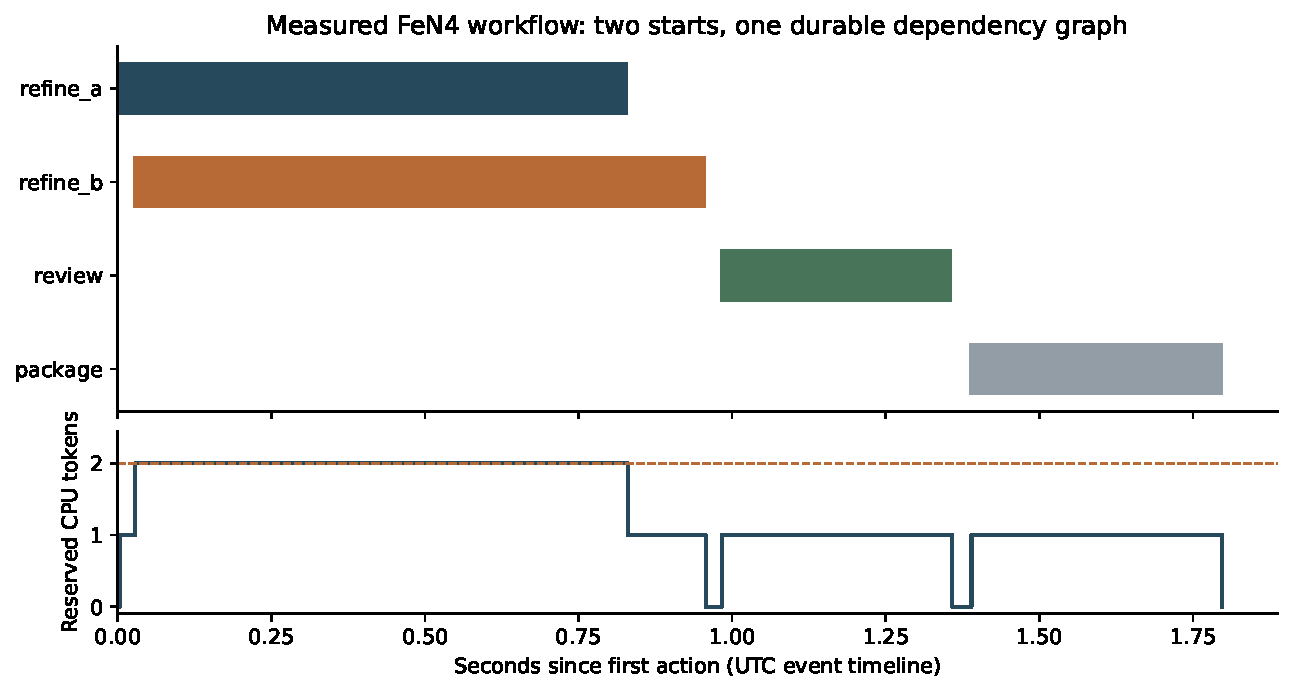
\includegraphics[width=0.96\textwidth]{figures/14_scheduler_timeline.pdf}
\caption{实际 FeN$_4$ 双起点工作流的调度时间线。色条包含解释器启动、计算和结果提交；两个精修动作同时存在，review 与 package 遵守依赖顺序。下图显示保留的 CPU 额度，不是操作系统测得的 CPU 利用率。时间线取自事件时间戳，执行预算使用单调时钟。}
\label{fig:scheduler-timeline}
\end{figure}
